% Created 2024-08-09 Fri 20:02
% Intended LaTeX compiler: pdflatex
\documentclass{article}
\usepackage[utf8]{inputenc}
\usepackage[T1]{fontenc}
\usepackage{graphicx}
\usepackage{longtable}
\usepackage{wrapfig}
\usepackage{rotating}
\usepackage[normalem]{ulem}
\usepackage{amsmath}
\usepackage{amssymb}
\usepackage{capt-of}
\usepackage{hyperref}

\usepackage{fancyhdr}
\usepackage[top=25mm, left=25mm, right=25mm]{geometry}
\usepackage{longtable}
\fancyhead[R]{}
\setlength\headheight{43.0pt}
\usepackage{listings}
\renewcommand{\lstlistingname}{Código}
\author{Profesor: Lenin G. Falconí M.Sc.}
\date{2024-08-07}
\title{Proyecto ICCD332 Arquitectura de Computadores}
\hypersetup{
 pdfauthor={Profesor: Lenin G. Falconí M.Sc.},
 pdftitle={Proyecto ICCD332 Arquitectura de Computadores},
 pdfkeywords={},
 pdfsubject={Proyecto de Fin de Semestre de la Materia de Arquitectura de Computadores},
 pdfcreator={Emacs 27.1 (Org mode 9.7.5)}, 
 pdflang={Spanish}}
\begin{document}

\maketitle
\tableofcontents

\fancyhead[C]{\includegraphics[scale=0.05]{../images/logoEPN.jpg}\\
ESCUELA POLITÉCNICA NACIONAL\\FACULTAD DE INGENIERÍA DE SISTEMAS\\
ARQUITECTURA DE COMPUTADORES}
\thispagestyle{fancy}
\section{City Weather APP}
\label{sec:orgff0555b}
Este es el proyecto de fin de semestre en donde se pretende demostrar
las destrezas obtenidas durante el transcurso de la asignatura de
\textbf{\textbf{Arquitectura de Computadores}}.

\begin{enumerate}
\item Conocimientos de sistema operativo Linux
\item Conocimientos de Emacs/Jupyter
\item Configuración de Entorno para Data Science con Mamba/Anaconda
\item Literate Programming
\end{enumerate}
\subsection{Estructura del proyecto}
\label{sec:orgaf53f15}
Se recomienda que el proyecto se cree en el \emph{home} del sistema
operativo i.e. \emph{home/<user>}. Allí se creará la carpeta \emph{CityWeather}
\begin{verbatim}
pwd
\end{verbatim}

El proyecto ha de tener los siguientes archivos y
subdirectorios. Adaptar los nombres de los archivos según las ciudades
específicas del grupo.

\begin{verbatim}
tree
\end{verbatim}

\begin{center}
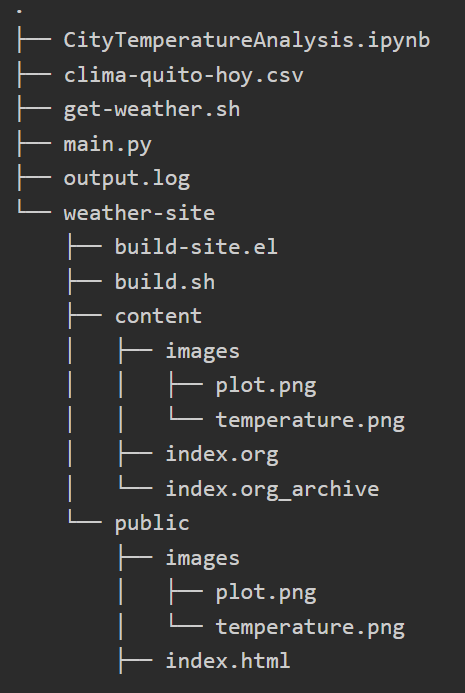
\includegraphics[height=0.5\textheight]{../images/projectDirectories.png}
\end{center}


Puede usar Emacs para la creación de la estructura de su proyecto
usando comandos desde el bloque de shell. Recuerde ejecutar el bloque
con \texttt{C-c C-c}. Para insertar un bloque nuevo utilice \texttt{C-c C-,} o \texttt{M-x
org-insert-structure-template}. Seleccione la opción \emph{s} para src y
adapte el bloque según su código tenga un comandos de shell, código de
Python o de Java. En este documento \texttt{.org} dispone de varios ejemplos
funcionales para escribir y presentar el código.

\begin{verbatim}
echo 'Aquí va sus comandos'
\end{verbatim}

\phantomsection
\label{org063ff70}
\begin{verbatim}
Aquí va sus comandos
\end{verbatim}
\subsection{Formulación del Problema}
\label{sec:org57b5f44}
Se desea realizar un registro climatológico de una ciudad
\(\mathcal{C}\). Para esto, escriba un script de Python/Java que permita
obtener datos climatológicos desde el API de \href{https://openweathermap.org/current\#one}{openweathermap}. El API
hace uso de los valores de latitud \(x\) y longitud \(y\) de la ciudad
\(\mathcal{C}\) para devolver los valores actuales a un tiempo \(t\).

Los resultados obtenidos de la consulta al API se escriben en un
archivo \emph{clima-<ciudad>-hoy.csv}. Cada ejecución del script debe
almacenar nuevos datos en el archivo. Utilice \textbf{crontab} y sus
conocimientos de Linux y Programación para obtener datos del API de
\emph{openweathermap} con una periodicidad de 15 minutos mediante la
ejecución de un archivo ejecutable denominado
\emph{get-weather.sh}. Obtenga al menos 50 datos. Verifique los
resultados. Todas las operaciones se realizan en Linux o en el
WSL. Las etapas del problema se subdividen en:

\begin{enumerate}
\item Conformar los grupos de 2 estudiantes y definir la ciudad
objeto de estudio.
\item Crear su API gratuito en \href{https://openweathermap.org/current\#one}{openweathermap}
\item Escribir un script en Python/Java que realice la consulta al
API y escriba los resultados en \emph{clima-<ciudad>-hoy.csv}. El
archivo ha de contener toda la información que se obtiene del
API en columnas. Se debe observar que los datos sobre lluvia
(rain) y nieve (snow) se dan a veces si existe el fenómeno.
\item Desarrollar un ejecutable \emph{get-weather.sh} para ejecutar el
programa Python/Java.\footnote{Recuerde que su máquina ha de disponer de un entorno de
anaconda/mamba denominado iccd332 en el cual se dispone del interprete
de Python}

\item Configurar Crontab para la adquisición de datos. Escriba el
comando configurado. Respalde la ejecución de crontab en un
archivo output.log
\item Realizar la presentación del Trabajo utilizando la generación
del sitio web por medio de Emacs. Para esto es necesario crear
la carpeta \textbf{\textbf{weather-site}} dentro del proyecto. Puede ajustar el
\emph{look and feel} según sus preferencias. El servidor a usar es
el \textbf{\textbf{simple-httpd}} integrado en Emacs que debe ser instalado:
\begin{itemize}
\item Usando comandos Emacs: \texttt{M-x package-install} presionamos
enter (i.e. RET) y escribimos el nombre del paquete:
simple-httpd
\item Configurando el archivo init.el
\end{itemize}

\begin{verbatim}
         (use-package simple-httpd
            :ensure t)
\end{verbatim}

Instrucciones de sobre la creación del sitio web se tiene en el
vídeo de instrucciones y en el archivo \href{https://github.com/LeninGF/EPN-Lectures/blob/main/iccd332ArqComp-2024-A/Proyectos/Org-Website.org}{Org-Website.org} en el
GitHub del curso

\item Su código debe estar respaldado en GitHub/BitBucket, la
dirección será remitida en la contestación de la tarea
\end{enumerate}
\subsection{Descripción del código}
\label{sec:orged70302}
En esta sección se debe detallar segmentos importantes del código
desarrollado así como la \textbf{\textbf{estrategia de solución}} adoptada por el
grupo para resolver el problema. Divida su código en unidades
funcionales para facilitar su presentación y exposición.

Lectura del API
\begin{verbatim}
def adder(a,b):
    return a+b
print(adder(5,3))
\end{verbatim}

Puede tener que borrar los dos puntos para que el resultado aparezca
en el HTML. En mi caso no fue necesario. Pruebe.
\phantomsection
\label{orge1b55a9}
\begin{verbatim}
8
\end{verbatim}


Convertir \emph{Json} a \emph{Diccionario} de Python
\begin{verbatim}
print(adder(8,8))
\end{verbatim}


Guardar el archivo csv
\begin{verbatim}
print(adder(8,-18))
\end{verbatim}
\subsection{Script ejecutable sh}
\label{sec:orgac6354d}
Se coloca el contenido del script ejecutable. Recuerde que se debe
utilizar el entorno de \textbf{\textbf{anaconda/mamba}} denominado \textbf{\textbf{iccd332}} para
la ejecución de Python; independientemente de que tenga una
instalación nativa de Python

En el caso de los shell script se puede usar `which sh` para conocer
la ubicación del ejecutable
\begin{verbatim}
which sh
\end{verbatim}

\phantomsection
\label{orgea4cea0}
\begin{verbatim}
/usr/bin/sh
\end{verbatim}


De igual manera se requiere localizar el entorno de mamba \textbf{iccd332}
que será utilizado

\begin{verbatim}
which mamba
\end{verbatim}

\phantomsection
\label{org5ab2057}
\begin{verbatim}
/home/leningfe/miniforge3/condabin/mamba
\end{verbatim}


Con esto el archivo ejecutable a de tener (adapte el código según las
condiciones de su máquina):

\begin{verbatim}
#!/usr/bin/sh
source /home/<user>/miniforge3/etc/profile.d/conda.sh
eval "$(conda shell.bash hook)"
conda activate iccd332
python main.py
\end{verbatim}

Finalmente convierta en ejecutable como se explicó en clases y laboratorio
\begin{verbatim}
#!/usr/bin/sh
Poner comando/s aquí
\end{verbatim}
\subsection{Configuración de Crontab}
\label{sec:orgb8403ce}
Se indica la configuración realizada en crontab para la adquisición de datos

\begin{verbatim}
*/t * * * * cd <City>Weather && ./get-weather.sh >> output.log 2>&1
\end{verbatim}

\begin{itemize}
\item Recuerde remplazar <City> por el nombre de la ciudad que analice
\item Recuerde ajustar el tiempo para potenciar tomar datos nuevos
\item Recuerde que \texttt{2>\&1} permite guardar en \texttt{output.log} tanto la salida
del programa como los errores en la ejecución.
\end{itemize}
\section{Presentación de resultados}
\label{sec:org9e7de3d}
Para la pressentación de resultados se utilizan las librerías de Python:
\begin{itemize}
\item matplotlib
\item pandas
\end{itemize}

Alternativamente como pudo estudiar en el Jupyter Notebook
\href{https://github.com/LeninGF/EPN-Lectures/blob/main/iccd332ArqComp-2024-A/Proyectos/CityWeather/CityTemperatureAnalysis.ipynb}{CityTemperatureAnalysis.ipynb}, existen librerías alternativas que se
pueden utilizar para presentar los resultados gráficos. En ambos
casos, para que funcione los siguientes bloques de código, es
necesario que realice la instalación de los paquetes usando \texttt{mamba
install <nombre-paquete>}
\subsection{Muestra Aleatoria de datos}
\label{sec:org37cb3cd}
Presentar una muestra de 10 valores aleatorios de los datos obtenidos.
\begin{verbatim}
import os
import pandas as pd
# lectura del archivo csv obtenido
df = pd.read_csv('/home/leningfe/PythonProjects/QuitoWeather/clima-quito-hoy-etl.csv')
# se imprime la estructura del dataframe en forma de filas x columnas
print(df.shape)
\end{verbatim}
\captionof{figure}{Lectura de archivo csv}

Resultado del número de filas y columnas leídos del archivo csv
\phantomsection
\label{orgc35387d}
\begin{verbatim}
(57, 30)
\end{verbatim}

\begin{verbatim}
table1 = df.sample(10)
table = [list(table1)]+[None]+table1.values.tolist()
\end{verbatim}
\captionof{figure}{Despliegue de datos aleatorios}

\begin{center}
\begin{tabular}{lrrllrlr}
dt & coord\textsubscript{lon} & coord\textsubscript{lat} & weather\textsubscript{0}\textsubscript{description} & \ldots{} & main\textsubscript{temp} & name & cod\\
\hline
2024-08-03 21:57:57 & -78.5249 & -0.2299 & overcast clouds & \ldots{} & 8.53 & Quito & 200\\
2024-08-04 10:26:16 & -78.525 & -0.2299 & overcast clouds & \ldots{} & 16.53 & Quito & 200\\
2024-08-04 09:15:02 & -78.5249 & -0.2299 & overcast clouds &  & 14.53 & Quito & 200\\
2024-08-06 10:05:50 & -78.5211 & -0.2309 & few clouds &  & 14.66 & Quito & 200\\
2024-08-03 02:43:26 & -78.5249 & -0.2299 & scattered clouds &  & 7.53 & Quito & 200\\
2024-08-04 22:50:26 & -78.5249 & -0.2299 & scattered clouds &  & 9.53 & Quito & 200\\
2024-08-03 12:52:29 & -78.5211 & -0.2309 & few clouds &  & 20.66 & Quito & 200\\
2024-08-03 10:54:26 & -78.5211 & -0.2309 & clear sky &  & 15.66 & Quito & 200\\
2024-08-02 23:51:42 & -78.5211 & -0.2309 & broken clouds &  & 8.66 & Quito & 200\\
2024-08-03 02:13:58 & -78.5249 & -0.2299 & scattered clouds &  & 7.53 & Quito & 200\\
\end{tabular}
\end{center}
\subsection{Gráfica Temperatura vs Tiempo}
\label{sec:orgda557fe}
Realizar una gráfica de la Temperatura en el tiempo.


El siguiente cógido permite hacer la gráfica de la temperatura vs
tiempo para Org 9.7+. Para saber que versión dispone puede ejecutar
\texttt{M-x org-version}

\begin{verbatim}
import matplotlib.pyplot as plt
import matplotlib.dates as mdates
# Define el tamaño de la figura de salida
fig = plt.figure(figsize=(8,6))
plt.plot(df['dt'], df['main_temp']) # dibuja las variables dt y temperatura
# ajuste para presentacion de fechas en la imagen 
plt.gca().xaxis.set_major_locator(mdates.DayLocator(interval=2))
# plt.gca().xaxis.set_major_formatter(mdates.DateFormatter('%Y-%m-%d'))  
plt.grid()
# Titulo que obtiene el nombre de la ciudad del DataFrame
plt.title(f'Main Temp vs Time in {next(iter(set(df.name)))}')
plt.xticks(rotation=40) # rotación de las etiquetas 40°
fig.tight_layout()
fname = './images/temperature.png'
plt.savefig(fname)
fname
\end{verbatim}

\begin{figure}[htbp]
\centering
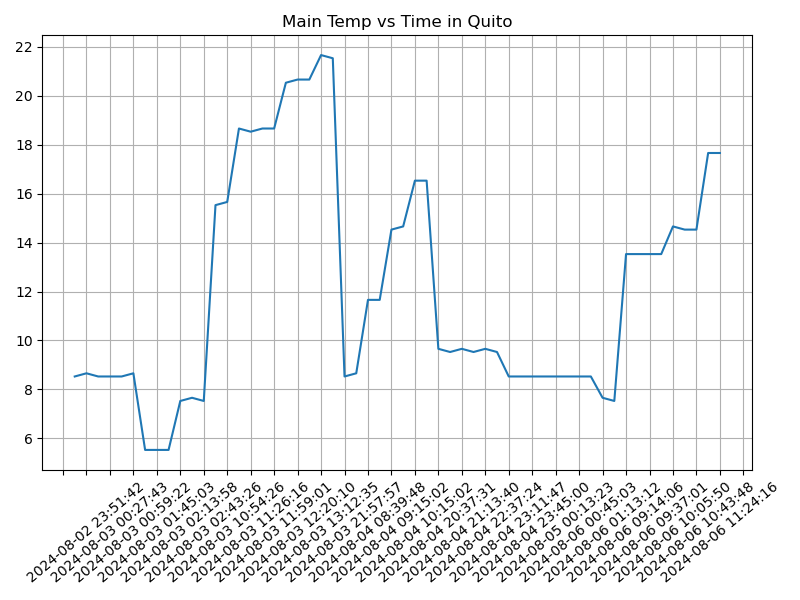
\includegraphics[width=.9\linewidth]{../images/temperature.png}
\caption{Gráfica Temperatura vs Tiempo}
\end{figure}

Debido a que el archivo index.org se abre dentro de la carpeta
\emph{content}, y en cambio el servidor http de emacs se ejecuta desde la
carpeta \emph{public} es necesario copiar el archivo a la ubicación
equivalente en \texttt{/public/images}

\begin{verbatim}
cp -rfv ./images/* /home/leningfe/PythonProjects/QuitoWeather/weather-site/public/images
\end{verbatim}
\subsection{Realice una gráfica de Humedad con respecto al tiempo}
\label{sec:orgb1dcdc1}
\subsection{\textbf{Opcional} Presente alguna gráfica de interés.}
\label{sec:org99a9f4a}
\section{Referencias}
\label{sec:org8b06e0d}
\begin{itemize}
\item \href{https://emacs.stackexchange.com/questions/28715/get-pandas-data-frame-as-a-table-in-org-babel}{presentar dataframe como tabla en emacs org}
\item \href{https://orgmode.org/worg/org-contrib/babel/languages/ob-doc-python.html}{Python Source Code Blocks in Org Mode}
\item \href{https://systemcrafters.net/publishing-websites-with-org-mode/building-the-site/}{Systems Crafters Construir tu sitio web con Modo Emacs Org}
\item \href{https://www.youtube.com/watch?v=AfkrzFodoNw}{Vídeo Youtube Build Your Website with Org Mode}
\end{itemize}
\end{document}
